\section{Introduction}

Brain is a network of $10^{10}$ neurons. Each neuron could generate a small electrical activity which alone could not be picked up from the electrodes. This is due to the interference of other surrounding activities. In case of a big number of neurons simultaneously active, the outcome signal is sufficiently high to be picked from the scalp electrodes. This electrical activity could be modeled as a dipole. Brain electrical activity has been investigated via surface electrodes since 1930. Widely known as electroencephalogram (EEG) is the potential difference of electrodes in a time course. This readings has facilitated the diagnoses of many neurological diseases. 

In simulation setup, dipole modeling could enable the generation of electrode potential via the solution of Poisson equation and Neuman boundary conditions. This is also known as the forward problem. Additionally, potential given the electrode, the underlying dipole localization and direction could also be estimated via different optimization setups. This is also known to be the inverse problem where the final outcome is source localization \cite{1}.

\section{Forward problem}

\subsection{Theory}
\subsubsection{Poisson's equation}

Poisson's equations computes the potentials distribution in a volume conductor given the applied current source. 
The current density $J(x,y,z)\big\{\frac{A}{m^2}\big\}$ is a vector field whereas its divergence defines the current source density $I_{m}=\nabla J\big\{\frac{A}{m^3}\big\}$. In case of a enclosed volume $r_{1}(x_{1},y_{1},z_{1})$ by current sink of positively charge represent the removal of positive ions. This yield a singularity current source density $-I\delta(r-r_{1})$. A small volume around the current source $r_{2}(x_{2},y_{2},z_{2})$ is also constructed. Injection of positively charge ions into this volume is also another singular current source density $I\delta(r-r_{2})$. Superposition of this cases outcome:
\begin{equation}\label{eq1}
   \nabla J= I\delta(r-r_{2})-I\delta(r-r_{1})
\end{equation}

As regard to the current density J and the electrical field E Ohm's law gives the relation via: 
\begin{equation}\label{eq2}
   J=E\sigma
\end{equation}

where $\sigma(r)$ is rank-1 tensor representation of the anisotropic conductivity which varies with the direction. Under the Faraday's law  in quasi-static conditions $(\nabla xE=0)$ a relation between the electrical field and scalar potential field is given via gradient operation:
\begin{equation}\label{eq3}
E=-\nabla V   
\end{equation}
The direction of $\nabla V$ represents the most rapid increase of the potential V at a give point. It sign  minus is based on the orientation flow from high to low potential. Poisson equation is obtained via combination of equations \ref{eq1}, \ref{eq2} and \ref{eq3}.

\begin{equation}\label{eq4}
\nabla (\sigma \nabla(V))=-I_{m}=I\delta(r-r_{2})-I\delta(r-r_{1})
\end{equation}

\subsubsection{Boundary conditions}

Inability to diminish charge particles at the compartments interface is seen as the current leaving one region is equal to the current entering another region. Additionally the very low conductivity of the human head does not permit any charge to penetrate the head. These two conditions presented by Neuman are equationed below:

\begin{figure}[!htbp]
\minipage{0.5\textwidth}%
\centering
\begin{equation}
    J_{1}e_{n}=J_{2}e_{n}
\end{equation}
\endminipage\hfill
\minipage{0.5\textwidth}%
\centering
\begin{equation}
    J_{1}e_{n}=0
\end{equation}
\endminipage\hfill
\end{figure}

\subsubsection{The current dipole}

The current source and sink remove the same amount of charges \textit{I} consequently dipole modeling is the best approach. Its momentum \textit{d} is defined via $d=I*p*e_{d}$ where $||d||=||I*p*e_{d}||$ and $e_{d}$ the orientation. Orthogonal projection of these dipole onto Cartesian axes is $d=d_{x}e_{x}+d_{y}e_{y}+d_{z}e_{z}$. Due to the linearity of Poisson equation it could be decomposed into:

\begin{equation}
    V(r,r_{dip},d)=d_{x}V(r,r_{dip},e_{x})+d_{y}V(r,r_{dip},e_{y})+d_{z}V(r,r_{dip},e_{z})
\end{equation}


\subsubsection{Solution of the forward problem}

Solution of the equation \ref{eq4} with gives the scalp potential at an electrode due to a singular dipole with momentum \textit{d}. A current dipole with momentum $d=de_{d}$ positioned at $r_{dip}$ in an infinite conductor with conductivity $\sigma_{i}$ produces a potential field at distance r as:

\begin{equation}
    V(r,r_{dip},d)=\frac{d(r-r_{dip})}{2\pi\sigma||r-r_{dip}||^3}
\end{equation}
which is also outlined in figure \ref{Fig7}
The easiest model to solve the Poisson equation for a head model is a the spherical head model which is fast and easy to be implemented. More sophisticated approaches are Boundary Element Method (BEM), Finite Element Method (FEM) and Finite Difference Method (FDM) which are generally employed for realistic shape instead of spherical which is not realistic. Due to the difference in conductivity of skull from scalp and brain a three shell concentric spherical head has to been proposed for spherical head model. Semi-analytic solution for Poisson equation utilizing the proposed geometrical modelling is:

\begin{equation}\label{eq11}
    V=\frac{1}{4\pi S R^2}\sum_{i=1}^{\infty}\frac{X(2i+1)^3}{g_{i}(i+1)i}b^{i-1}\{id_{r}P_{i}(cos\theta)+id_{r}P_{i}(cos\theta)\}
\end{equation}
given that:
\begin{equation}
    g_{i}=\{(i+1)X+i\}\{\frac{iX}{i+1}+1\}+(1-X)\{(i+1)X+i\}(f_{1}^{i_{1}}-f_{2}^{i_{1}})-i(1-X)^2\{\frac{f_{1}}{f_{2}}\}^2
\end{equation}
where:



\begin{figure}[!htbp]
\minipage{0.5\textwidth}%
    \centering
\begin{itemize}
    \item $d_{r}$ is the radial component
    \item $d_{t}$ is the tangential component 
    \item R is the radius of the outer shell
    \item S is the conductivity of the scalp and brain tissue
    \item X is the ratio between the skull and soft tissue conductivity 
    \item b is the relative distance of the dipole from the center
    \item $\phi$ is the polar angle of the surface point    
\end{itemize}
\endminipage\hfill
\minipage{0.5\textwidth}%
    \centering    
\begin{itemize}
     \item $P_{i}(.)$ is the Legendre polynomial
    \item $P^{1}_{i}(.)$ is the associated Legendre polynomial
    \item \textit{i} is an index
    \item $i_{1}=2*i+1$
    \item $r_{1}$ is the radius of the inner shell
    \item $r_{2}$ is the radius of the middle shell
    \item $f_{1}=\frac{r_{1}}{R}$ 
    \item $f_{2}=\frac{r_{2}}{R}$    
\end{itemize}
\endminipage\hfill
\end{figure}


This is the equation for scalp potentials produced from an dipole located in the z axis. In case of an of an arbitrary dipole, Euler angles are employed for the rotation of the coordinate system accordingly. 

\subsection{EEG montage}

Electrode placement is of great importance to display the EEG adequately. There is a big diversity of EEG montage which in same cases it should be adopted for specific applications. The most accepted model is 10/20 for classical EEG recording. There are symmetric placement between Nasion-Inion marked as Frontal pole $(F_{p}$, Central (C), Parietal (P), occipital (O) and Temporal T. The electrodes named with zero (Z) are the ones corresponding at the central line. The odd numbers are used for points on the left hemisphere whereas the even number for points on the right of the hemisphere. There is a symmetry of the node placement respectively to the Nassion-Ion line \ref{Fig1}. 

\begin{figure}[!htbp]
\minipage{0.35\textwidth}%
    \centering
    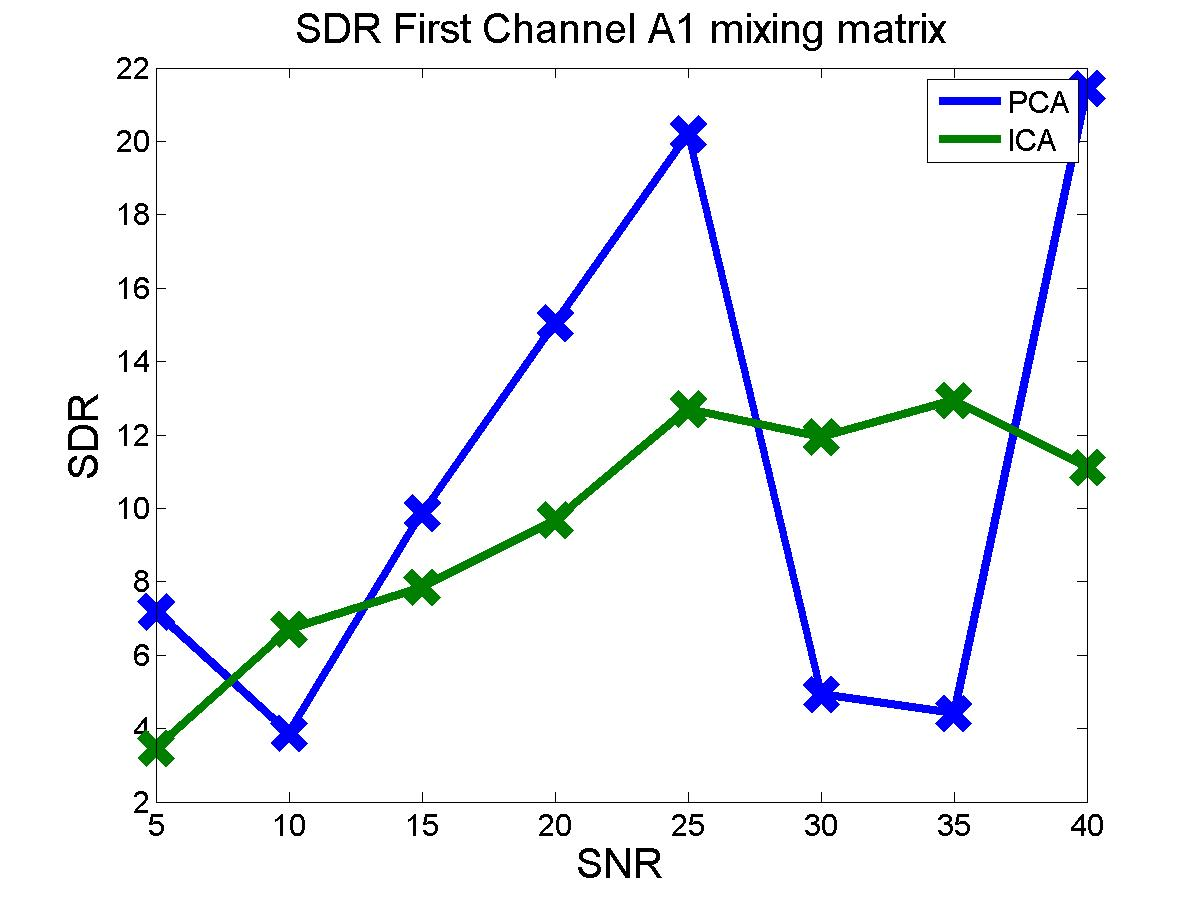
\includegraphics[width=1\textwidth]{1.jpg}
    \subcaption{Epical view}
\endminipage\hfill
\minipage{0.5\textwidth}%
    \centering
    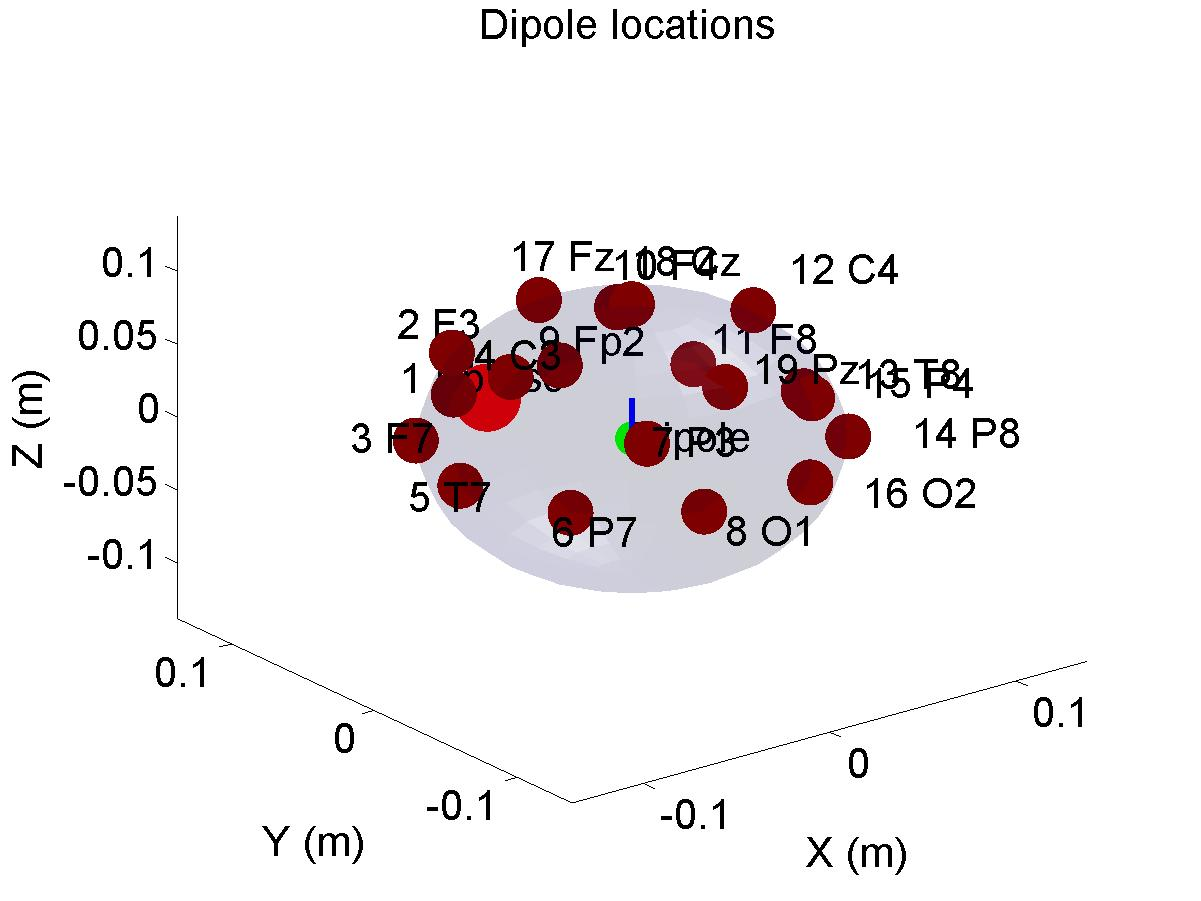
\includegraphics[width=1\textwidth]{2.jpg}
    \subcaption{3D view}
\endminipage\hfill
\caption{EEG montage for the simulation model}\label{Fig3}
\end{figure}


In figure \ref{Fig3} is the spherical model which will be used as well as the electrode placement as the most standard configuration. The spherical model we are using consist o a three shell model figure \ref{Fig4} with respective radius:

\begin{figure}[!htbp]
\minipage{0.33\textwidth}%
    \centering
\begin{itemize}
    \item $R_{skull}=0.08[m]$
\end{itemize}
\endminipage\hfill
\minipage{0.33\textwidth}%
    \centering
\begin{itemize}
    \item $R_{scalp}=0.086[m]$
\end{itemize}
\endminipage\hfill
\minipage{0.33\textwidth}%
    \centering
\begin{itemize}
    \item $R_{brain}=0.092[m]$
\end{itemize}
\endminipage\hfill
\end{figure}


\subsection{Dipole location}

The modeled dipole has two main parameters position and direction which are encoded into Cartesian coordinates. In figure \ref{Fig5} a simple dipole location at the center which is oriented towards z axis. This is acquired via command line $Show-Dipole-Placement([0,0,0,0,0,1],hm,4)$ where $Show-Dipole-Placement([x_{p},y_{p},z_{p},Ori_{x},Ori_{y},Ori_{z}],Head-Model,Nr_{Figure})$. In case it would be necessary to place an dipole half way from the center towards the right ear oriented towards z axis figure \ref{Fig6} that would be possible via command $Show-Dipole-Placement([0.05,0,0,0,0,1],hm,5)$.

\begin{figure}[!htbp]
\minipage{0.5\textwidth}%
    \centering
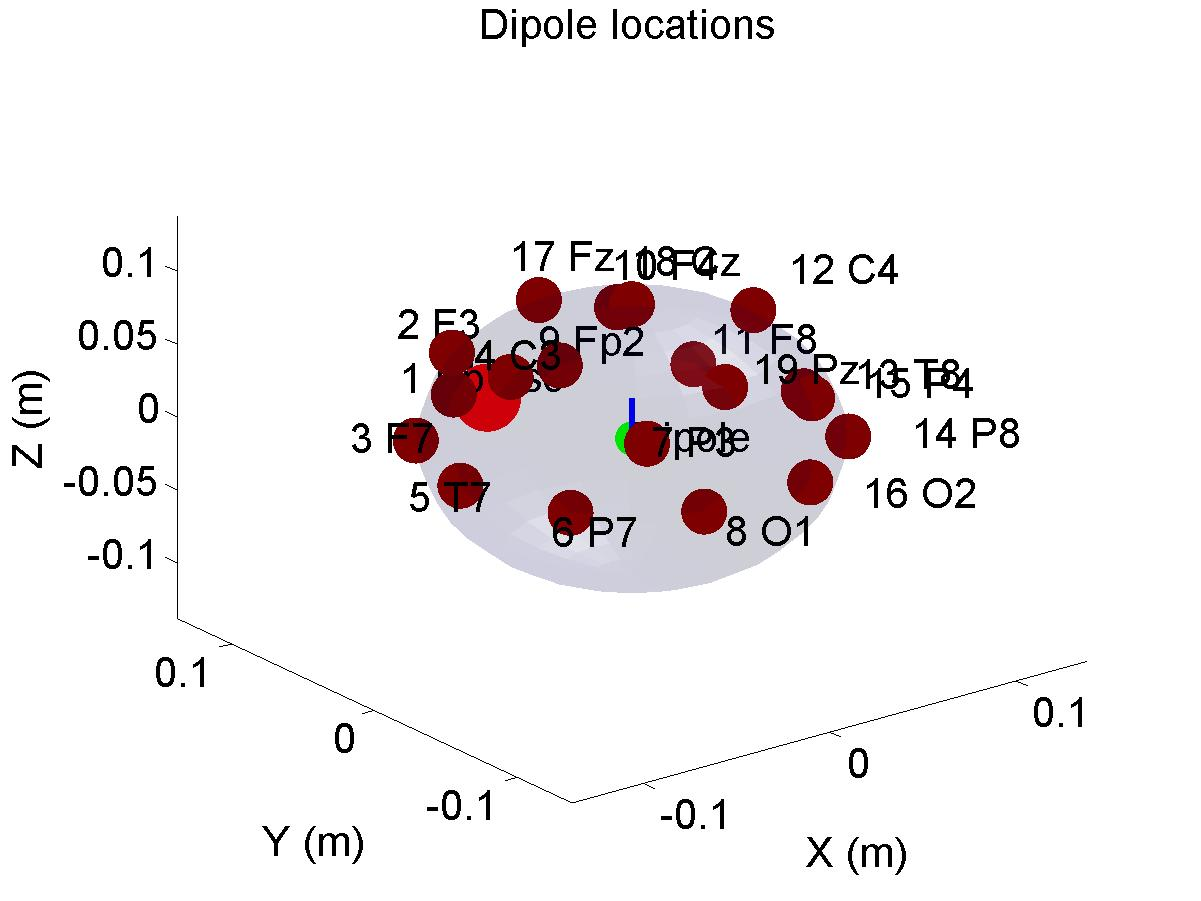
\includegraphics[width=1\textwidth]{2.jpg}
\subcaption{Dipole modeled in the center}\label{Fig5}
\endminipage\hfill
\minipage{0.5\textwidth}%
    \centering
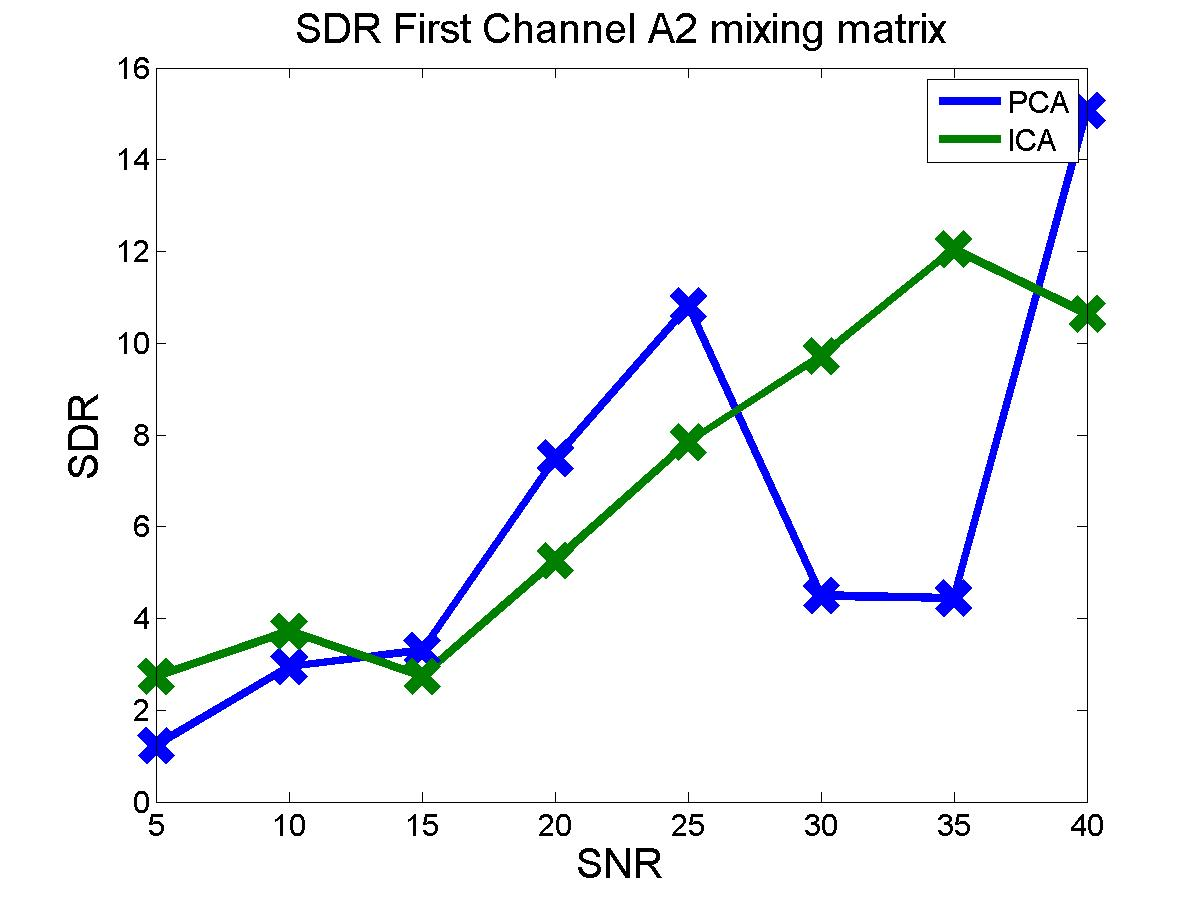
\includegraphics[width=1\textwidth]{3.jpg}
\subcaption{Dipole located halfway from center to the right ear.}\label{Fig6}
\endminipage\hfill
\caption{Dipole locations}
\end{figure}



\subsubsection{Potential computation}

Spherical head model has been utilized to solve the Poisson equations and provides the potential distribution at particular coordinate due a dipole at particular direction and position. In case there will be a dipole located in the center oriented towards the \textit{x} position the potential field distribution will be as in the figure \ref{Fig9}. Since the dipole is not positioned along the z axis from \cite{2} are all the necessary transformation needed to for the coordinates rotation which are also outlined in Appendix \ref{Ap1}. The generalization of equation \ref{eq11} for any dipole location can be written as:


\begin{figure}[!htbp]
\minipage{0.33\textwidth}%
    \centering
\begin{equation}\label{ldf1}
    V_{x}=T_{x}D_{x}
\end{equation}
\endminipage\hfill
\minipage{0.33\textwidth}%
    \centering
\begin{equation}\label{ldf2}
    V_{y}=T_{y}D_{y}
\end{equation}
\endminipage\hfill
\minipage{0.33\textwidth}%
    \centering
\begin{equation}\label{ldf3}
    V_{z}=T_{z}D_{z}
\end{equation}
\endminipage\hfill
\caption{Voltage computation}\label{new_label1}
\end{figure}

whereas the potential V at $R_{2}$ due to dipole D located at $R_{1}$ is: $V=V_{x}+V_{y}+V_{z}$. Regarding the electrode potential values the plot in figure \ref{Fig10} outline individual values. The dipole location and orientation is plotted in figure \ref{Fig11}. The potential field is therefore mostly oriented towards the right ear in the figure \ref{Fig9} which coincides with the orientation of the dipole inside the head. 

\begin{figure}[!htbp]
\minipage{0.33\textwidth}%
    \centering
    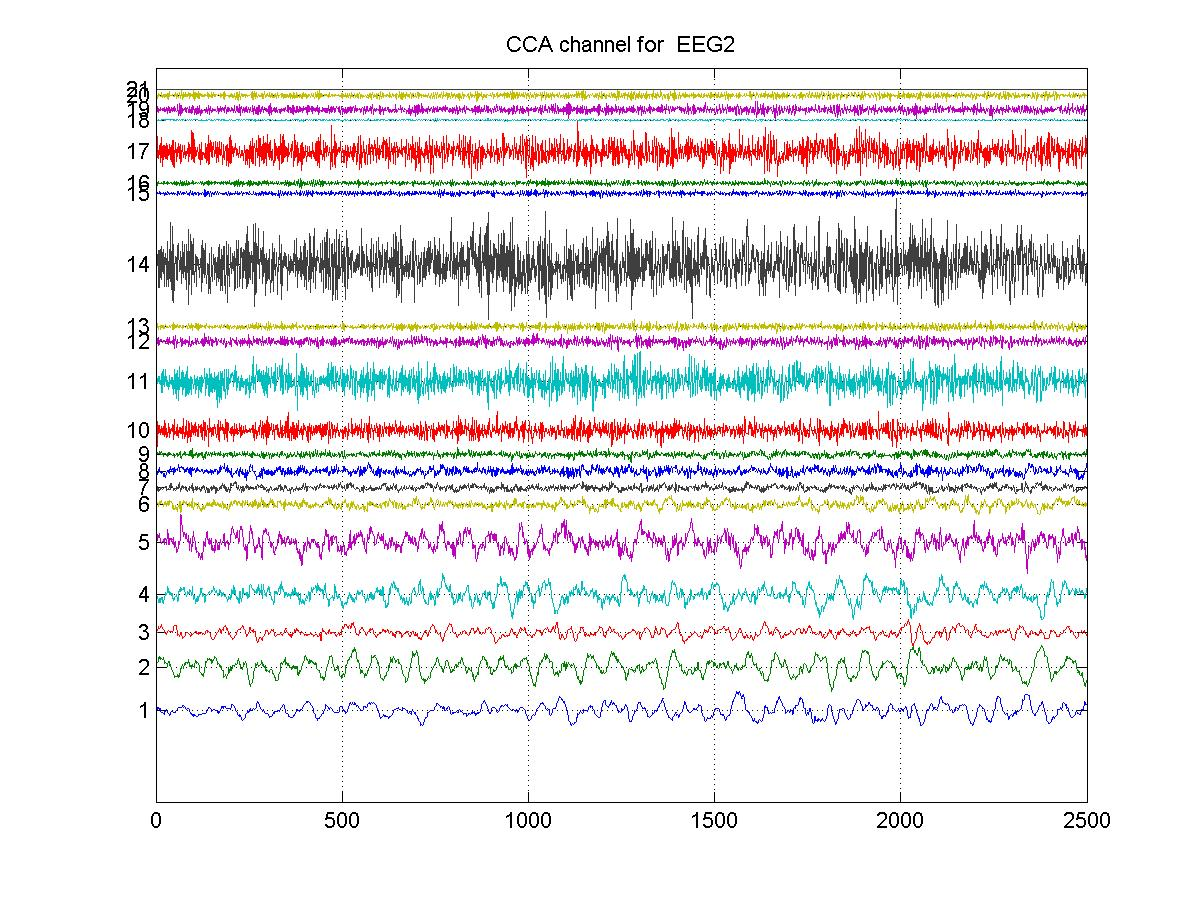
\includegraphics[width=1\textwidth]{4.jpg}
    \subcaption{Potential distribution.}\label{Fig9}
\endminipage\hfill
\minipage{0.33\textwidth}%
    \centering
    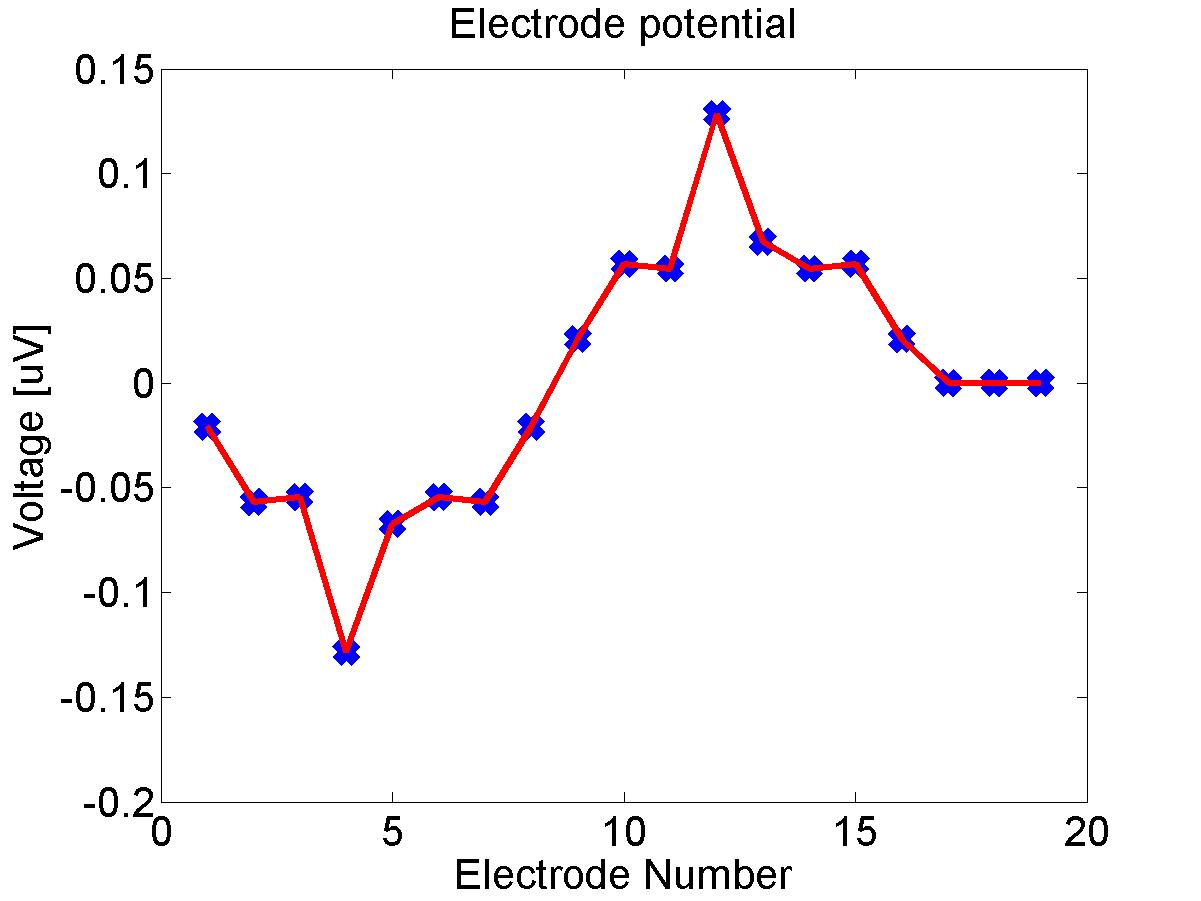
\includegraphics[width=1\textwidth]{5.jpg}
    \subcaption{Potential at each electrode.}\label{Fig10}
\endminipage\hfill
\minipage{0.33\textwidth}%
    \centering
    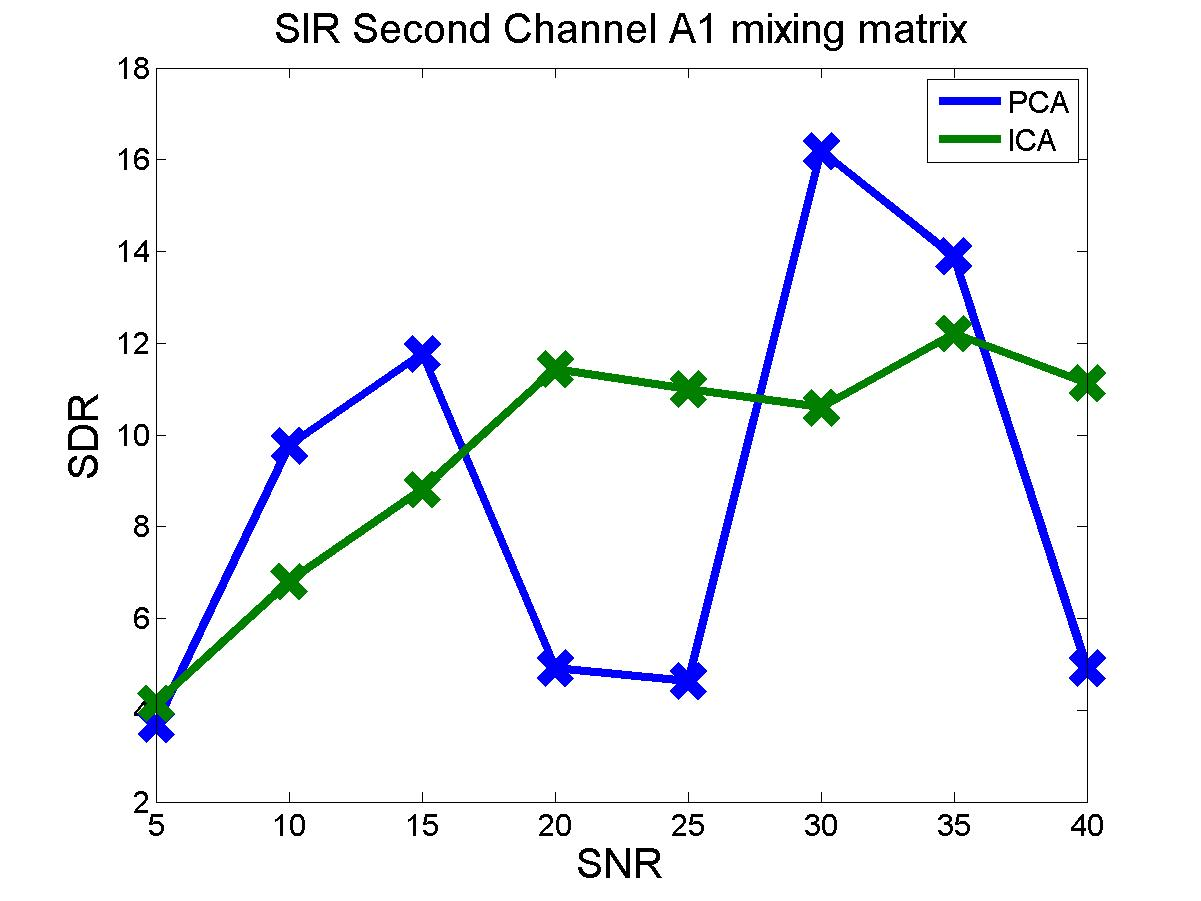
\includegraphics[width=1\textwidth]{6.jpg}
    \subcaption{Dipole location.}\label{Fig11}
\endminipage\hfill
\caption{Potential distribution}
\end{figure}

\newpage
\subsection{Lead Field Matrix}

The lead field matrix contains the potential intensity computed from the spherical model, oriented along x, y and z axis. The final potential distribution corresponding to the a particular dipole orientation is the superposition of each lead field matrix along each axis, whereby their contribution is proportional to the orientation of the dipole. 
In figure \ref{LFM} are the potential distribution of each component where it is clearly noted maximum along X,Y and Z axis. 

\begin{figure}[!htbp]
\minipage{0.33\textwidth}%
    \centering
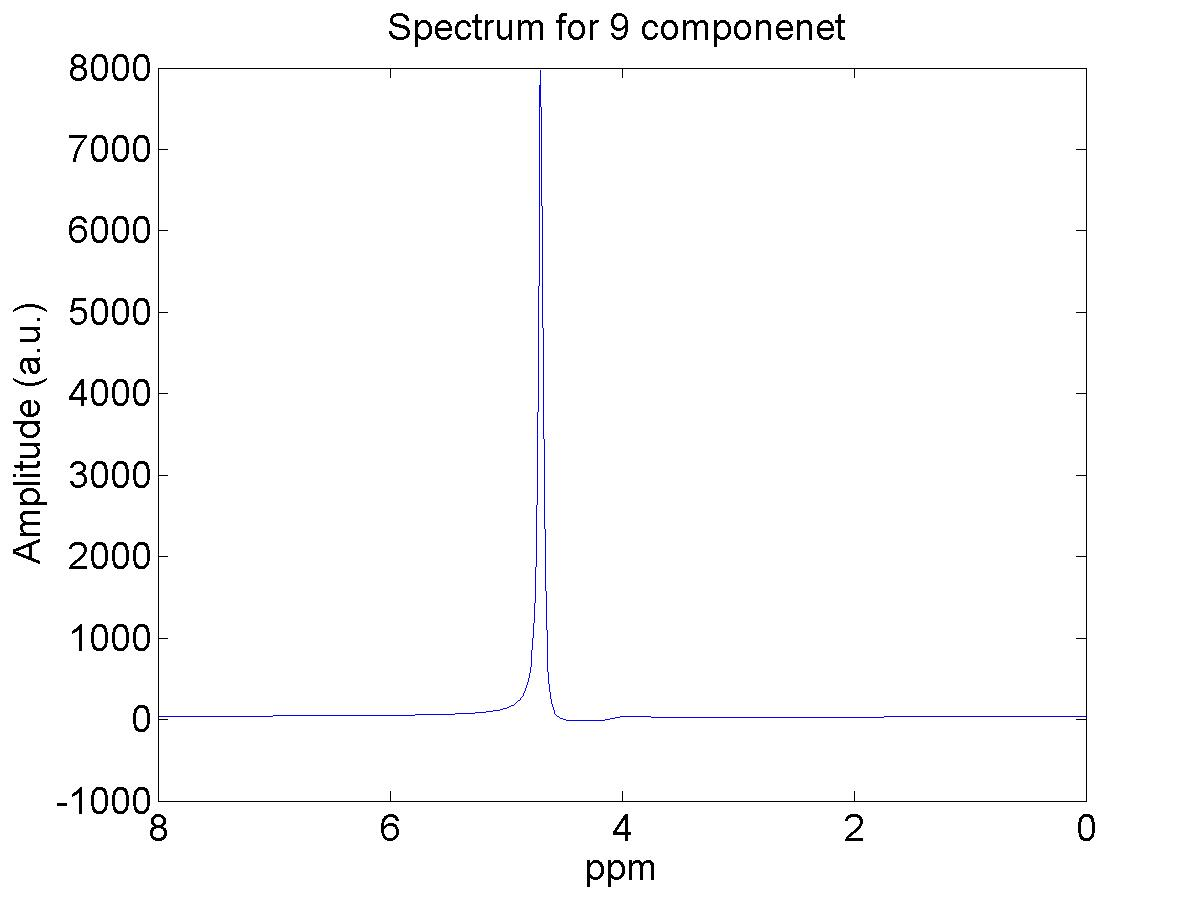
\includegraphics[width=1\textwidth]{7.jpg}
\subcaption{Potential generated along x}
\endminipage\hfill
\minipage{0.33\textwidth}%
    \centering
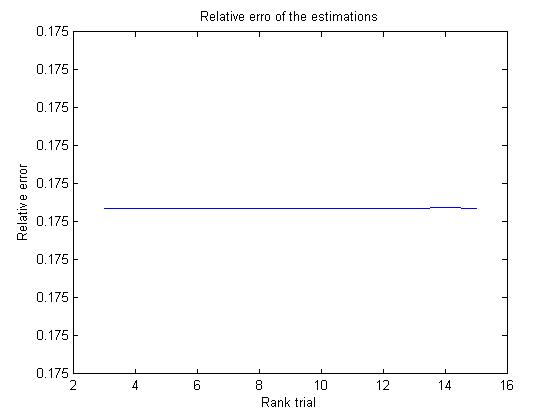
\includegraphics[width=1\textwidth]{8.jpg}
\subcaption{Potential generated along y}
\endminipage\hfill
\minipage{0.33\textwidth}%
    \centering
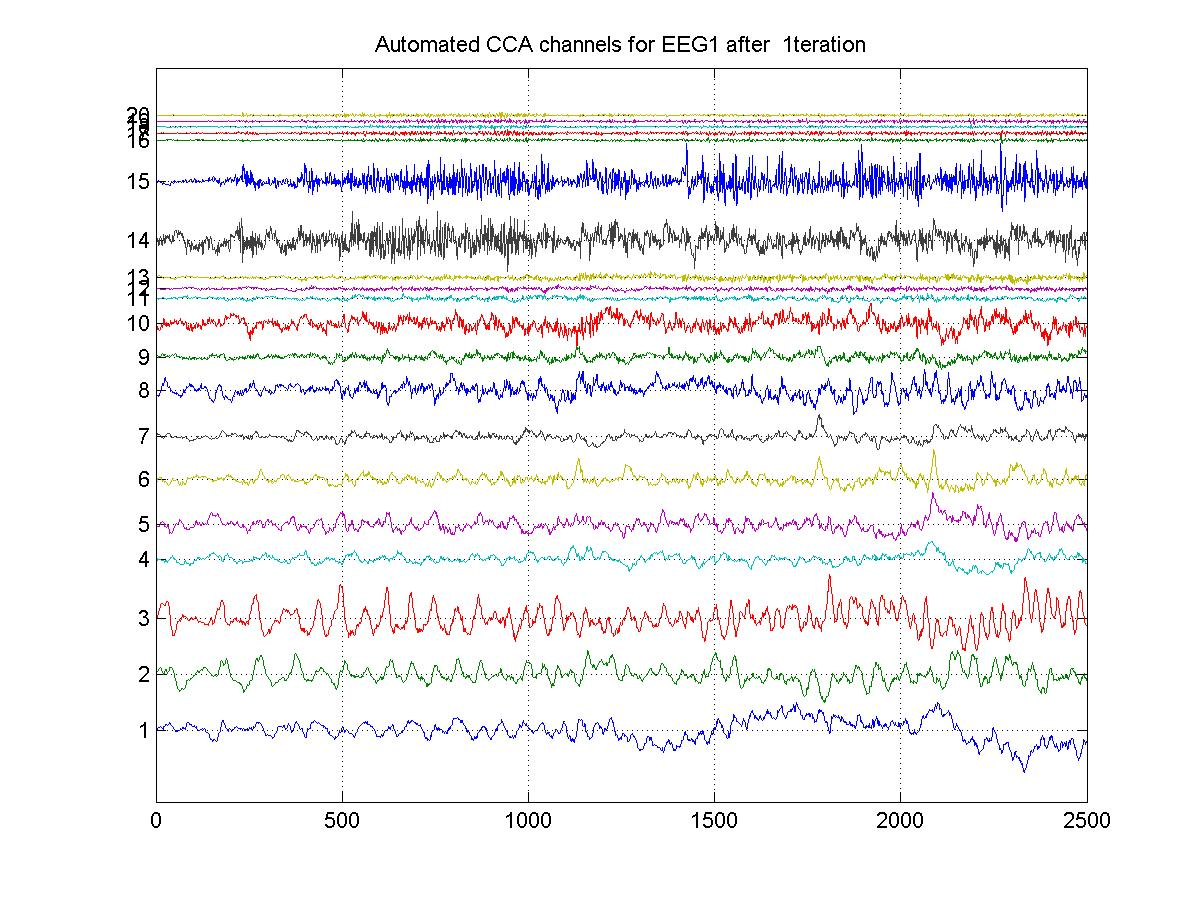
\includegraphics[width=1\textwidth]{9.jpg}
\subcaption{Potential generated along z}
\endminipage\hfill
\caption{Lead field matrix}\label{LFM}
\end{figure}


\newpage
\subsection{Linearity of Maxwell equation}

The numerical verion of the Maxwel equation is linear therefore the principle of superposition is applied. Therefore in this case, the potential produced from the dipole D1 and D2 located at the center where the first one oriented along \textit{x} \ref{D1} and the second one along \textit{z} in figure \ref{D2} produces the potentials in figure \ref{pote1} and figure \ref{pote2}. Due to the linearity the final potential from these two dipole will be as in figure \ref{FinalPotential}. Differently this potential would be excactly the same as the potential distribution outcomed from a single dipole where the orientation is the vectorial sum of dipole D1 and D2 figure \ref{D3}. This equality is also testified from dipole distributions in figure \ref{Testified}.


\begin{figure}[!htbp]
\minipage{0.5\textwidth}%
    \centering
    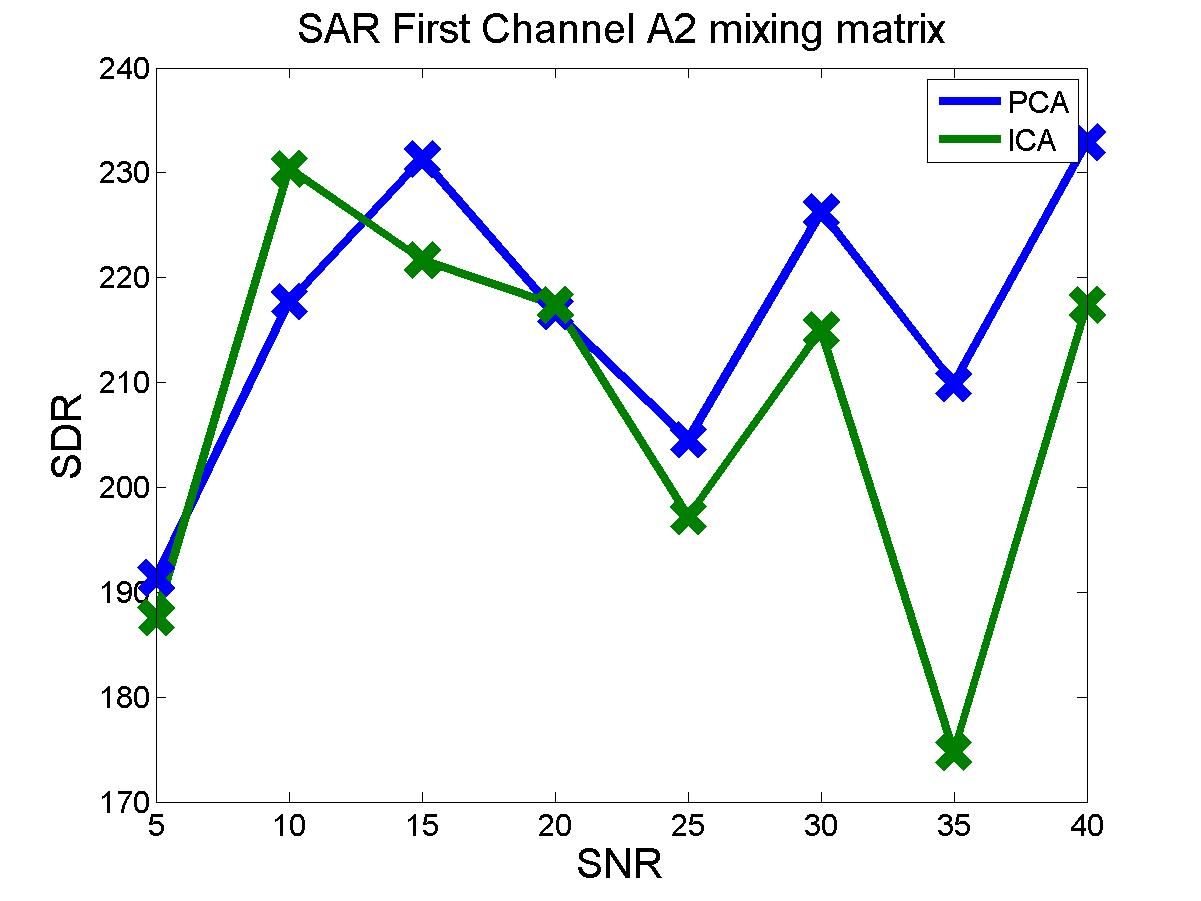
\includegraphics[width=1\textwidth]{11.jpg}
    \subcaption{Voltage from dipole oriented along x}\label{pote1}
\endminipage\hfill
\minipage{0.5\textwidth}%
    \centering
    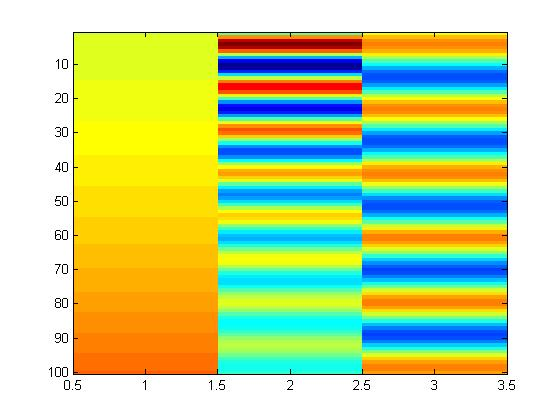
\includegraphics[width=1\textwidth]{12.jpg}
    \subcaption{Voltage from dipole oriented along y}\label{pote2}
\endminipage\hfill
\caption{Voltage distribution}
\end{figure}



\begin{figure}[!htbp]
\minipage{0.33\textwidth}%
    \centering
    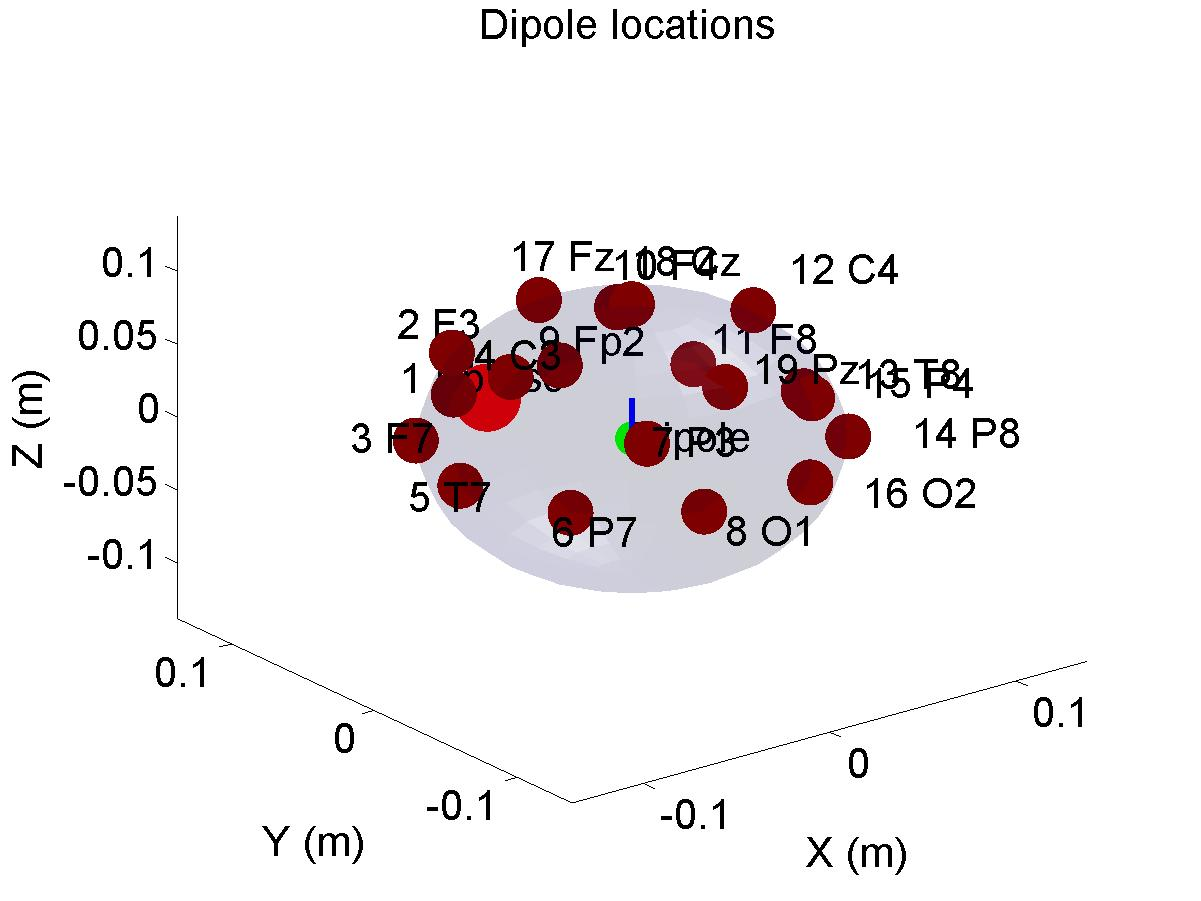
\includegraphics[width=1\textwidth]{14.jpg}
    \subcaption{Dipole along x}\label{D1}
\endminipage\hfill
\minipage{0.33\textwidth}%
    \centering
    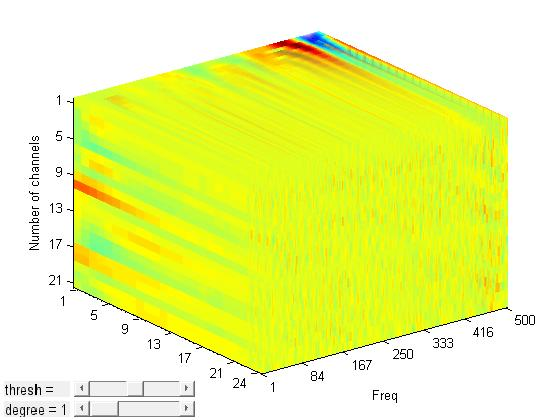
\includegraphics[width=1\textwidth]{15.jpg}
    \subcaption{Dipole along z}\label{D2}
\endminipage\hfill
\minipage{0.33\textwidth}%
    \centering
    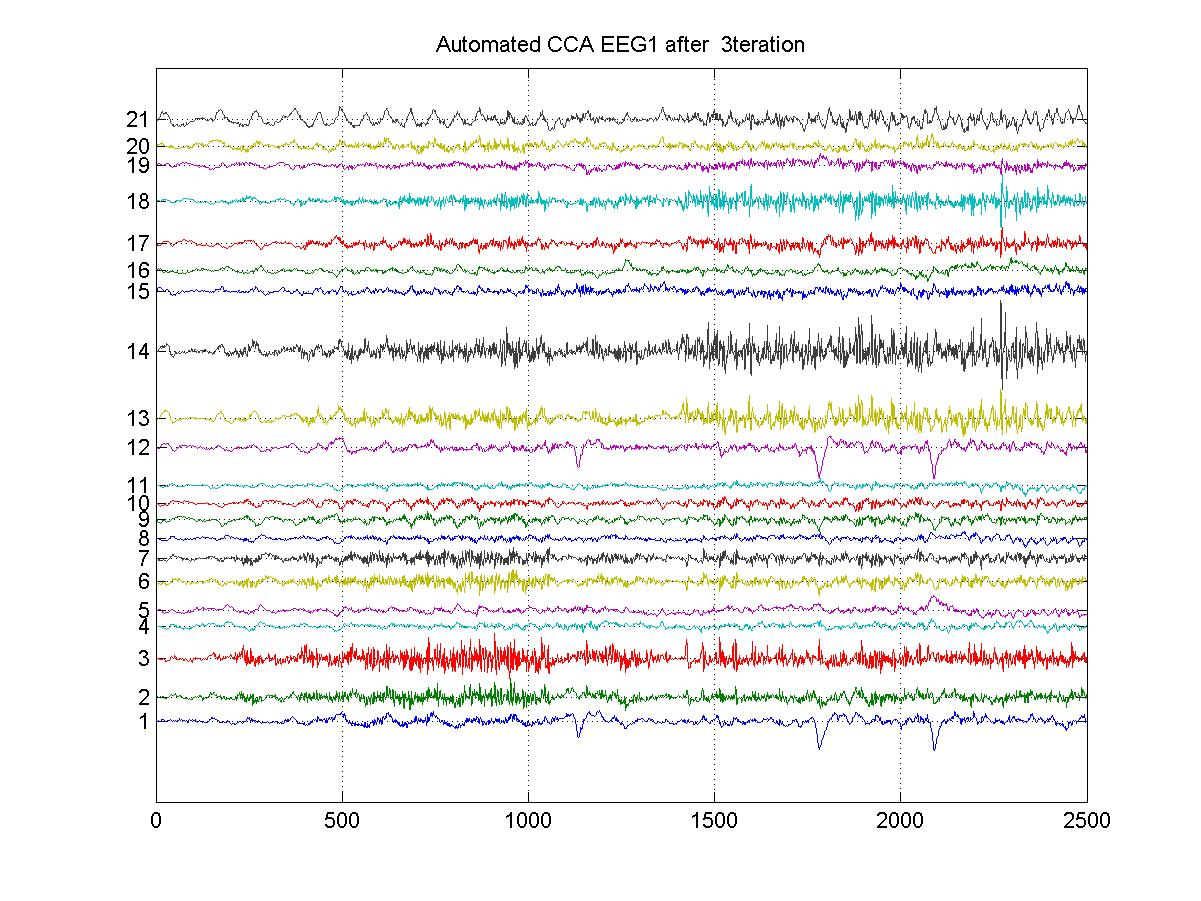
\includegraphics[width=1\textwidth]{16.jpg}
    \subcaption{Dipole with orientation along xz}\label{D3}
\endminipage\hfill
\caption{Dipole location}
\end{figure}



\begin{figure}[!htbp]
\minipage{0.5\textwidth}%
    \centering
    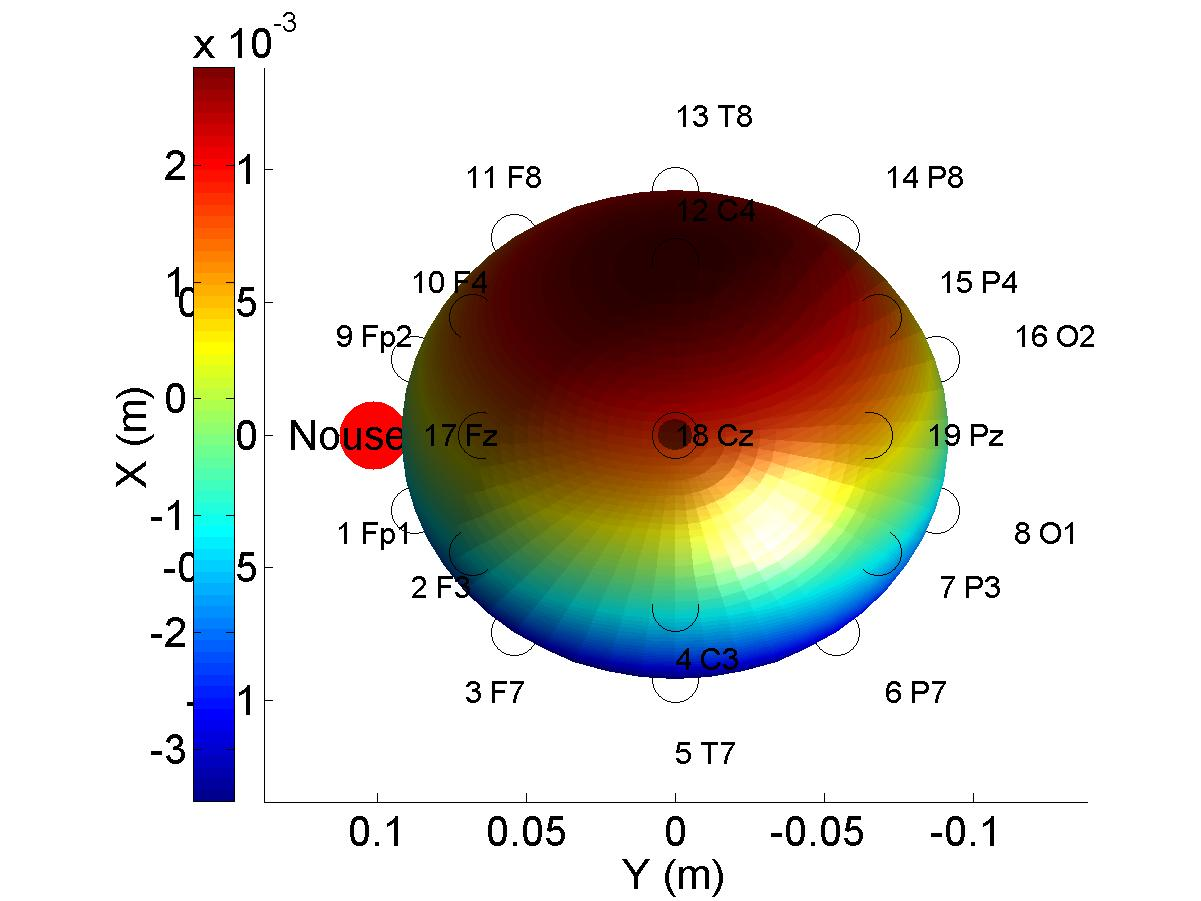
\includegraphics[width=1\textwidth]{10.jpg}
    \subcaption{Voltage superposition}\label{FinalPotential}
\endminipage\hfill
\minipage{0.5\textwidth}%
    \centering
    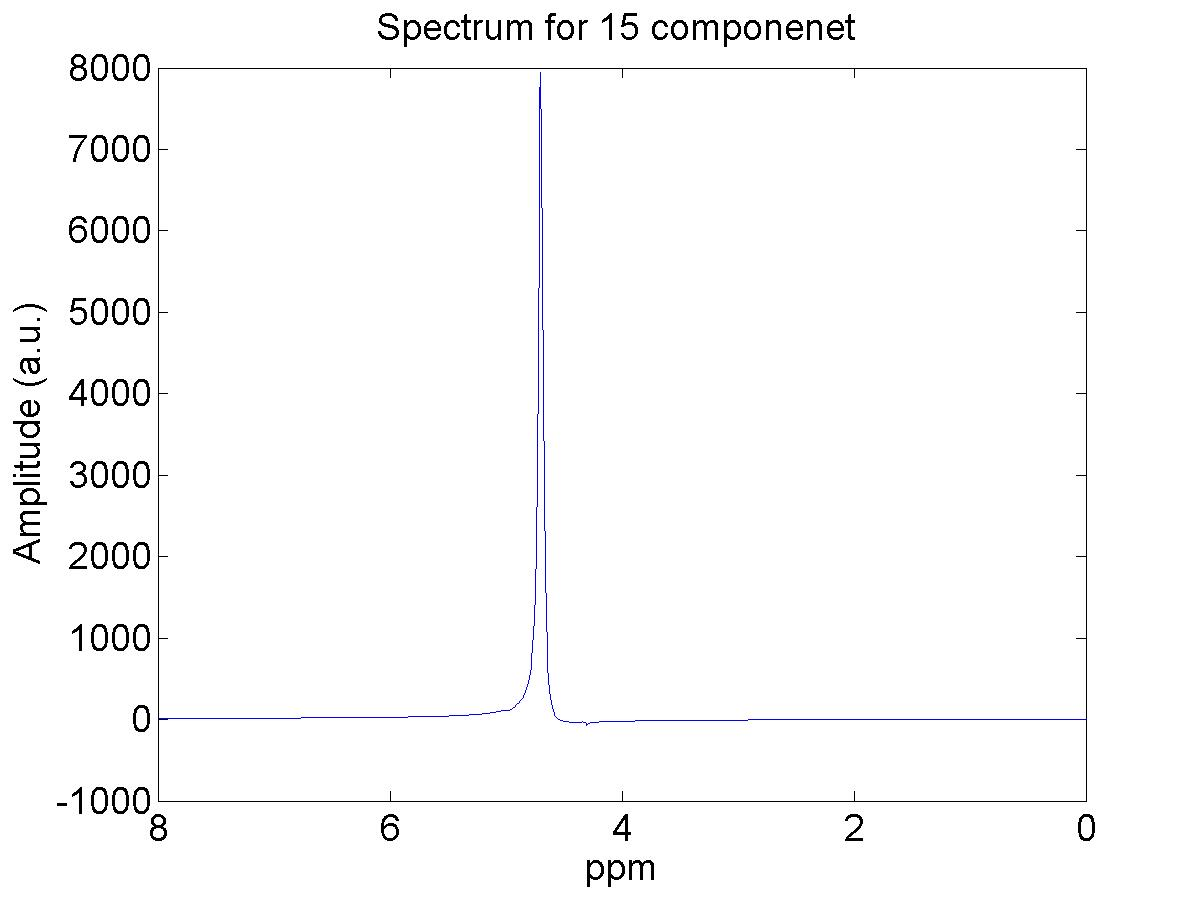
\includegraphics[width=1\textwidth]{13.jpg}
    \subcaption{Voltage from the dipole along xy} \label{figure_1}
\endminipage\hfill
\caption{Potential distribution}\label{Testified}
\end{figure}


\newpage
\subsection{EEG time series generation}

Hereby EEG time series are being simulated by rotating along the xy plane the dipole located in the coordinates (0,-0.05,0.02) figure \ref{D5}. The sampling frequency is 200 Hz which is much higher than the dipole rotation frequency which is 10 Hz in our case. After 3 sec EEG simulation from the time series values plotted in figure \ref{EEG} what can be observed is that the electrodes near the dipole has a much higher amplitude comparing to the ones sitting further from the dipole.



\begin{figure}[!htbp]
\minipage{0.5\textwidth}%
    \centering
    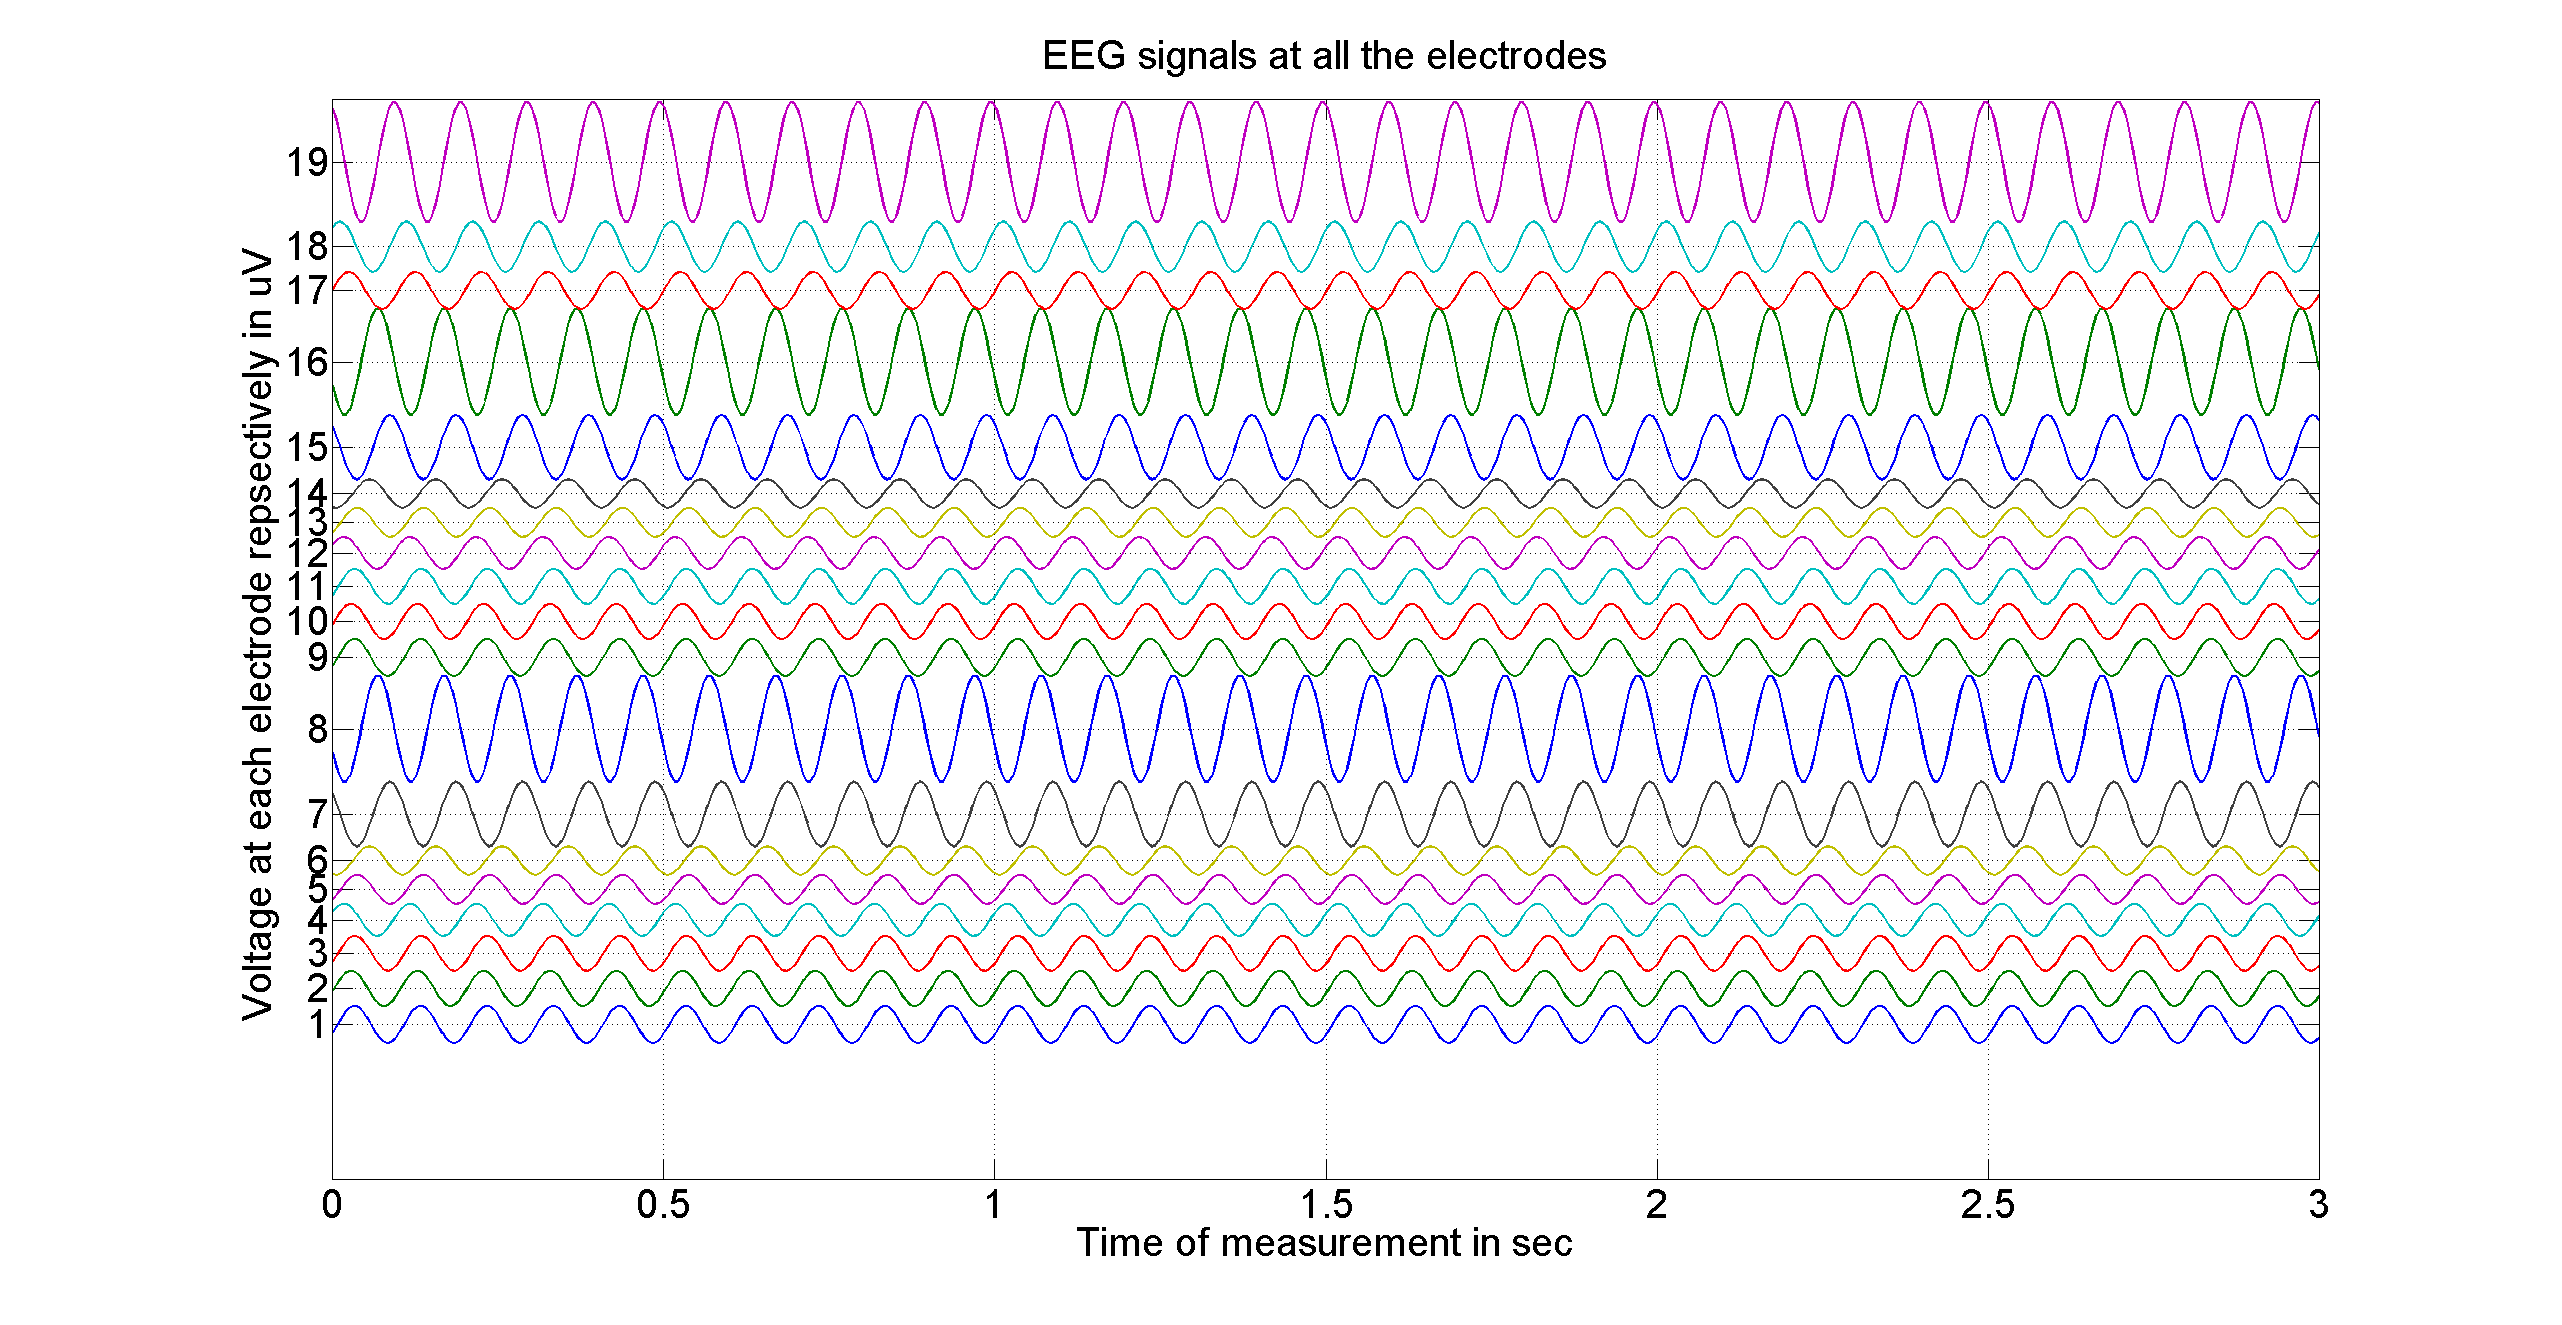
\includegraphics[width=1\textwidth]{17.png}
    \subcaption{EEG plot}\label{EEG}
\endminipage\hfill
\minipage{0.5\textwidth}%
    \centering
    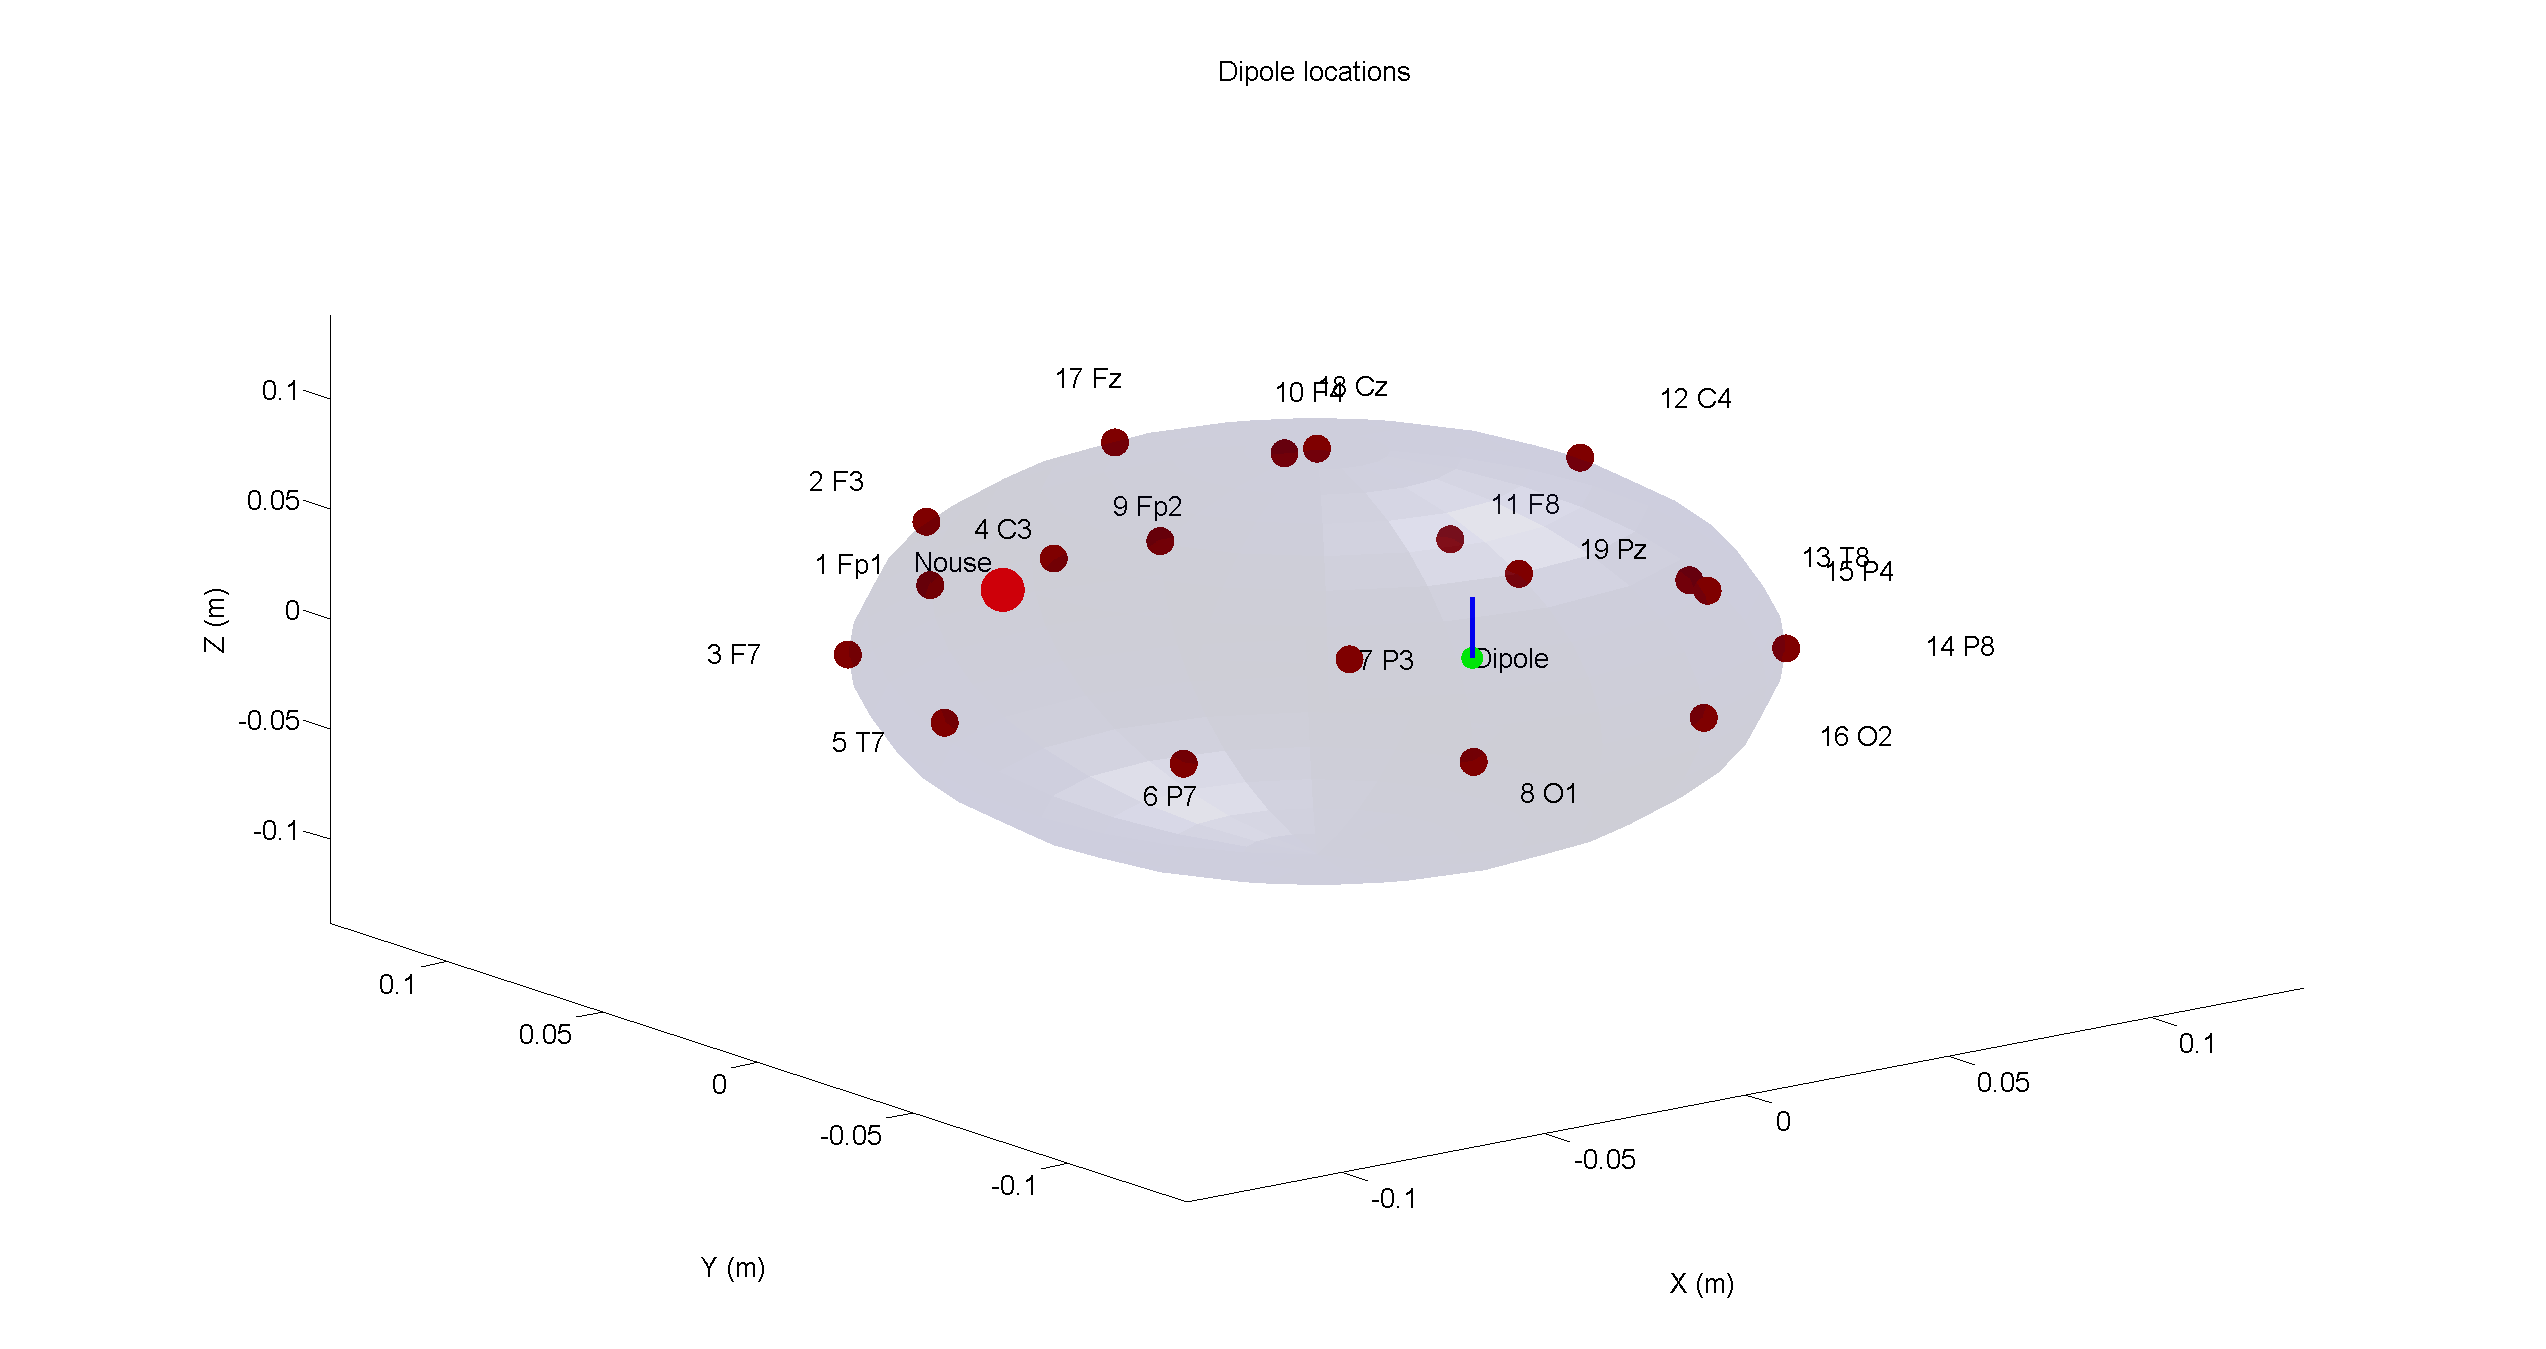
\includegraphics[width=1\textwidth]{18.png}
    \subcaption{Dipole}\label{D5}
\endminipage\hfill
\caption{EEG simulation}
\end{figure}
